\section{Software prototyping}
\subsection{Embedded development environment}

Software shoud take care of the motor control, IMU output readings and remote control, this could create complications, as essentially they would interrupt each other. A way of multitasking should be introduced.
"An RTOS (Real-Time Operating System) is a software component that lets you rapidly switch between different running sections of your code. Think of it as having several loop() functions in an Arduino sketch where they all run at the same time." \cite{Joe2019}

After research, the list was narrowed to two top condenders – FreeRTOS and Zephyr. Both solutions are open source, widely used and support the Microcontroller board we have chosen. \cite{Lemberg}
According to 2018 IoT Developer Survey \cite{IOT}, FreeRTOS is one of the most popular OS used and while Zephyr only received a 2.8 \% rating in 2018, it is often described as one of the fastest growing RTOS and in 2022 has become the largest open-source RTOS project by the number of commits and developers. (See Figure~\ref{fig:iot_os})
\begin{figure}[H]
    \centering
    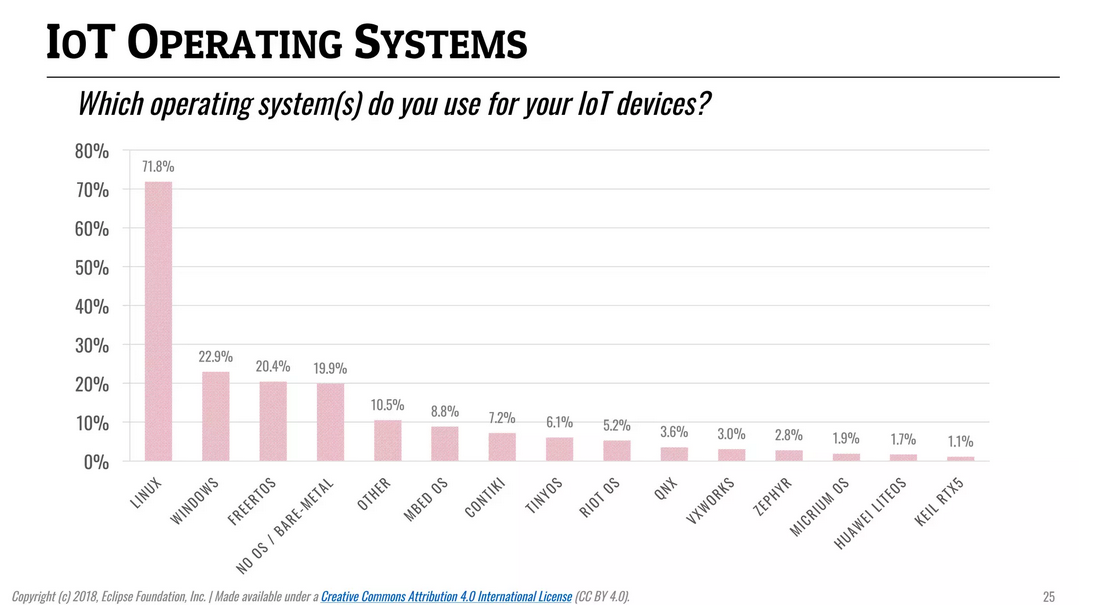
\includegraphics[scale = 0.5]{pictures/iot_os.PNG}
    \caption{IoT Developer Survey 2018 results}
    \label{fig:iot_os}
\end{figure}

To decide between the RTOS choice, a pros and cons table was created and evaluated. \cite{Comparison} (See Table~\ref{table.rtos})

\begin{table}[H]
      \makegapedcells
  \setlist[itemize]{font=\color{black},
                    nosep,
                    leftmargin=*,
                    after=\vspace*{-\baselineskip}}
      \setlength{\tabcolsep}{3pt}
  \begin{tabularx}{\linewidth}{|>{\RaggedRight}p{25mm}|*{2}{I |}}
      \hline
  RTOS
      &   \mcl{Advantages}    &   \mcl{Disadvantages}        \\
      \hline
  FreeRTOS 
      &   \item Suitable for begginers
          \item Constantly improved
          \item Fast code execution
          \item Low memory consuption
          &   \item Not event-driven (scheduler will only be called once in a certain period of time)
              \item Less flexible
              \\
      \hline
  ZephyrRTOS
      &   \item Constantly improved
          \item Designed to ensure energy efficiency
          \item Highly configurable
          \item Event-driven
          \item Kernel can create additional system threads
          \item Possible to exclude multithreading
          \item Additional debugging features
          \item Supported by Nordic Semiconductor
          &   \item More difficult to set-up
              \item Potentially complicated to use with no experience
              \\
      \hline

\end{tabularx}
\caption{Comparison between ZephyrRTOS and FreeRTOS}
\label{table.rtos}
\end{table}

Overall FreeRTOS is better established and would be easier to use, in case of no experience, whereas Zephyr offers more flexibility and is a fast growing solution, well suited for our application and would be a worthwile investment for building our skillset. \cite{Industry}
After setting up a embedded environment for software development with ZephyrRTOS. (See appendix \ref{zephyr}), it was conducted, that the use of ZephyrRTOS is possible.
After further consultation with the supervisors, it was conducted, that there is a lack of skill in RTOS, more specifically in threading. With the guidence of Davi, it was concluded, that acquiring such skills would be outside the scope of the project, as the main focus is control engineering.
In conclusion, the choice was made to use Arduino IDE with the Arduino framework, with the chance of switching to Mbed OS, if a need arises for it.